\documentclass{article}
\usepackage{amsmath}
\usepackage{mathtools}
\usepackage{amssymb}
\usepackage{graphicx}

\title{Regressão Linear: Implementação e Teoria}
\author{
    Glauco Fleury
}
\date{}

\begin{document}
\maketitle

\section{Introdução à Regressão Linear}
 
Trata-se em suma de um modelo de 'curve fitting': dado
um domínio que apresenta diversas features, isto é,
tem um número $D$ de características (representado
matematicamente por vetores $x \in \mathbb{R}^{D} $), e
uma imagem $y$ a qual se deseja estimar com a função,
o objetivo é encontrar uma curva a qual melhor se encaixe
nos dados já presentes, de modo que seja possível utilizar
a função que a descreve para tentar predizer resultados 
futuros.

A regressão linear assume que a função buscada terá o
seguinte formato: 

\begin{equation}
    \begin{split}
        f(x, \theta) &=  \theta_{0} + \theta_{1}x_{1} + \theta_{2}x_{2}
        + ... + \theta_{D}x_{D} \\ 
        &= \theta \cdot x
    \end{split}
\end{equation}

Isto é, ela assume que a variável a ser prevista pode ser
entendida como a combinação linear das dimensões do vetor de 
input. Do modo como está escrita, a função buscada será 
necessariamete, uma reta (2D), plano (3D), ou qualquer tipo de
hiperplano para mais dimensões. 

\subsection{Ruído e Probabilidade}

Considerando $y = \hat{y} + \epsilon = f(x,\theta) + \epsilon$,
sendo $\epsilon$ o ruído intrínseco à coleta de dados e 
$f(x,\theta) = \hat{y}$ a melhor previsão do modelo acerca do
real resultado, torna-se necessária a abordagem estatística
sobre a modelagem da regressão. Ela toma o seguinte formato:

\begin{equation}
    p(y|x,\theta) \rightarrow y \sim \mathcal{N}(x \cdot \theta, \sigma^{2}) 
\end{equation}

O que basicamente significa que assumimos que a chance de 
$\hat{y}$ "acertar" $y$ é dada por uma distribuição normal,
em que a maior parte das vezes ele acerta, mas pode errar,
porém a estimativa tem chances menores de cometer erros quanto
mais absurdos eles são.

Considerando que o ruído $\epsilon$
advém de uma função de densidade de probabilidade normal,
com média 0 (a maior parte das vezes, $\epsilon = 0$) e
desvio padrão = $\sigma$, podemos escrever que $\epsilon \sim
\mathcal{N}(0, \sigma^{2})$. A variança dessa normal é 
idêntica à outra devido ao fato do ruído ser o fator comum 
de variação em ambos os casos.

\section{Maximum Likelihood Estimation}

Maximum Likelihood Estimation se resume a buscar o vetor de 
parâmetros $\theta_{MLE}$ tal que a curva descrita melhor se 
adeque aos dados, parametrizando-a de modo a encaixá-la nos
pontos do espaço $\mathbb{R}^{D}$. Para isso, é desejável
maximizar a probabilidade de que cada resultado $y$ advenha
de nosso modelo probabilístico (cuja média nós definiremos
com $f(x,\theta) = x^{T}\theta$). Em resumo, buscamos
(para um número $N$ de vetores $x$):

\begin{align}
    \theta_{MLE} &= \underset{\theta}{\arg\max} 
    \prod_{n=1}^{N} p(y_{n}|x_{n}, \theta) \\
    &= \underset{\theta}{\arg\max} \prod_{n=1}^{N}
    \mathcal{N}(y|x \cdot \theta, \sigma^{2}) \\
    &= \underset{\theta}{\arg\min} 
    - \Sigma_{n=1}^{N} \log (\mathcal{N}
    (y|x \cdot \theta, \sigma^{2}))
\end{align}

Sabe-se que $\mathcal{N}(\mu, \sigma^{2}) = 
\frac{1}{\sigma \sqrt{2\pi}} e^{-\frac{1}{2}
(\frac{x - \mu}{\sigma})^{2}}$, e, portanto, é possível
rescreever $\theta_{MLE}$ na forma:

\begin{align}
    \theta_{MLE} &= \underset{\theta}{\arg\min}[ 
    -N\log(\sigma) -\frac{N}{2}\log(2\pi)
    -\frac{1}{2\sigma^{2}}\Sigma_{n=1}^{N}
    (y_{n} - x_{n}^{T}\theta)^{2}] \\
    &= \underset{\theta}{\arg\min} [
    -\frac{1}{2\sigma^{2}}\Sigma_{n=1}^{N}
    (y_{n} - x_{n}^{T}\theta)^{2}]
\end{align}

Para facilitar, vamos escrever o somatório na forma matricial,
e também igualar a equação acima a uma função, de tal forma
que:

\begin{equation}
    \theta_{MLE} = \underset{\theta}{\arg\min} [L(\theta)]
\end{equation}
\begin{equation}
    L(\theta) = -\frac{1}{2\sigma^{2}}
    ||(Y - X\theta)||^{2}
\end{equation}

Onde $X = [x_{1}, x_{2}, ..., x_{n}]^{T}$ e 
$Y = [y_{1}, y_{2}, ..., y_{n}]^{T}$ .

A partir daqui, para achar o nosso parâmetro, fica claro que
o problema se torna a minimazação de uma função quadrada. Como
a Hessiana de $L(\theta)$ é positiva e semi-definida, fica claro
que estamos lidando com um problema de otimização convexa, ou
seja, é possível encontrar uma solução óptima. 

Efetuando $\frac{dL}{d\theta} = 0$ (tal qual ensinam em cálculo I),
encontra-se uma fórmula para a otimização:

\begin{equation}
    \theta_{MLE} = (X^{T}X)^{-1}X^{T}Y
\end{equation}

O problema com essa fórmula está em encontrar a matriz inversa.
O algoritmo atual mais rápido para tal apresenta complexidade
$O(n^{3})$, o que é sub-óptimo, para dizer o mínimo. Como 
alternativa, é possível utilizar um método iterativo que aproxime
nosso tão sonhado vetor de parâmetros. Nesse projeto, escolhi
particularmente o famoso "gradient descent" para estimar os
valores desconhecidos.

\subsection{Expansão Polinomial}

Como eu havia dito no começo, esse modelo de regressão linear
é limitado pela presença de formas lineares (hiperplanos) para
descrever nossas previsões. Observe o seguinte caso, por exemplo:

\begin{figure}[h!]
    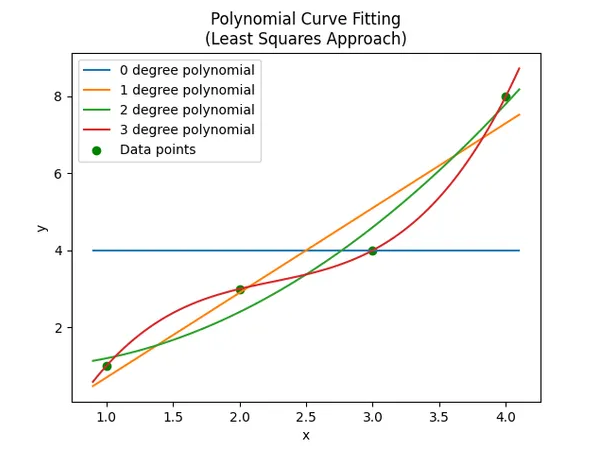
\includegraphics[width=9cm, height=7cm]{pool.png}
    \centering
    \caption{modelagem com diferentes graus de polinômios}
  \end{figure}

Claramente a reta não é adequada para tentar descrever o 
padrão descrito pelos dados. A solução? Expandir polinomialmente
as dimensões analisadas, a fim de capturar padrões mais 
complexos. A isso damos o nome de "polynomial expansion", uma
forma de inclusão de features.

Formalmente, o que buscamos é uma forma de construir um novo
vetor, chamado de feature vector ($\phi(x)$), o qual mudará
o domínio de nossa função para incluir dimensões não lineares.
A função resultante permanece uma combinação linear de dimensões,
já que todos os parâmetros tem grau 1. Desse modo, para
um feature vector qualquer: $\phi(x): \mathbb{R}^{D} \rightarrow
\mathbb{R}^{K}$

O feature vector utilizado nesse projeto é conhecido como
"expansão polinomial": ele expande o vetor $x$ para incluir
combinações de grau maior de seus componentes. Dessa forma,
se $x = [x_{1}, x_{2}, ..., x_{n}]^{T}$:

\begin{equation}
    \phi(x) = [CR(x_{1}, x_{2}, ..., x_{n})]^{T} 
\end{equation}

CR é uma sigla para combinação com reposição. Por exemplo, para
$x = [x_{1}, x_{2}]^{T}$ com grau 2 de expansão, e 
$x' = [x_{1}]$ com grau 5, teremos, respectivamente:

\begin{equation}
    \phi(x) = [x_{1}, x_{2}, x_{1}^{2}, x_{1}x_{2}, x_{2}^{2}]^{T} 
\end{equation}

\begin{equation}
    \phi(x') = [x_{1}, x_{1}^{2}, x_{1}^{3}, x_{1}^{4}, x_{1}^{5}]^{T} 
\end{equation}

Dessa maneira, é possível realizar justamente o que  figura 
anterior exibe: criar curvas com curvatura não nula, que se
adequem melhor à descrição do problema, encontrando agora 
um vetor de pesos $\theta \in \mathbb{R}^{K}$. 

\subsection{Regularização}
 
O que acontece quando nosso modelo é perfeito para os dados
que utilizamos? Digamos que, para $K$ pontos de dados que eu
tenha, eu crie uma função com $K$ dimensões; nesse caso, o modelo
terá uma dimensão $x_{k}$ para cada ponto $P_{k}$, e acabará
por passar precisamente por todos estes pontos perfeitamente,
tornando $L(\theta) = 0$. O problema com isso é a perda de 
generalidade: o modelo "decorou" o caso utilizado para treiná-lo,
e, em qualquer outro conjunto de pontos fornecidos que advenham
da mesma distribuição-fonte desse caso, ele terá uma 
performance horrível.

\begin{figure}[h!]
    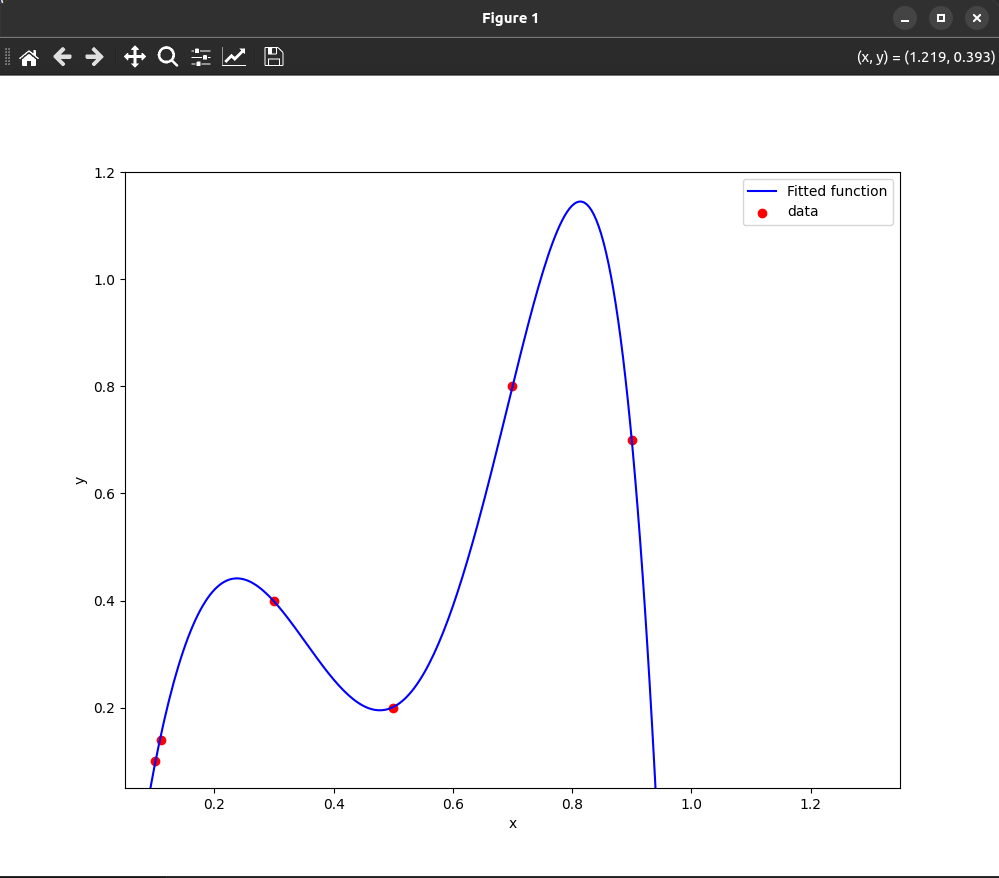
\includegraphics[width=9cm, height=7cm]{overfit.png}
    \centering
    \caption{exemplo de overfitting; $10^{6}$ epochs, e 
    learning factor = $0.1$}
  \end{figure}

Mesmo que haja menos dimensões comparado ao número de pontos,
o modelo ainda pode generalizar muito mal. A fim de prevenir
ainda mais isso, introduz-se o bridge-regularization term, 
somando à loss function um termo que penaliza a adição de 
parâmetros muito elevados:

\begin{equation} \label{eq:14}
    L(\theta, \lambda) = -\frac{1}{2\sigma^{2}}
    ||(Y - X\theta)||^{2} + \lambda
    ||\theta||_{2}^{2}
\end{equation}

Onde $\lambda$ é o coeficiente de aprendizado ("Learning Rate"),
proporcional ao quanto queremos punir nosso modelo por 
overfitting, e o $2$ embaixo do módulo de $\theta$ simboliza
a norma euclidiana (é possível utilizar outras também, mas 
foi essa a que eu usei).

\begin{figure}[h!]
    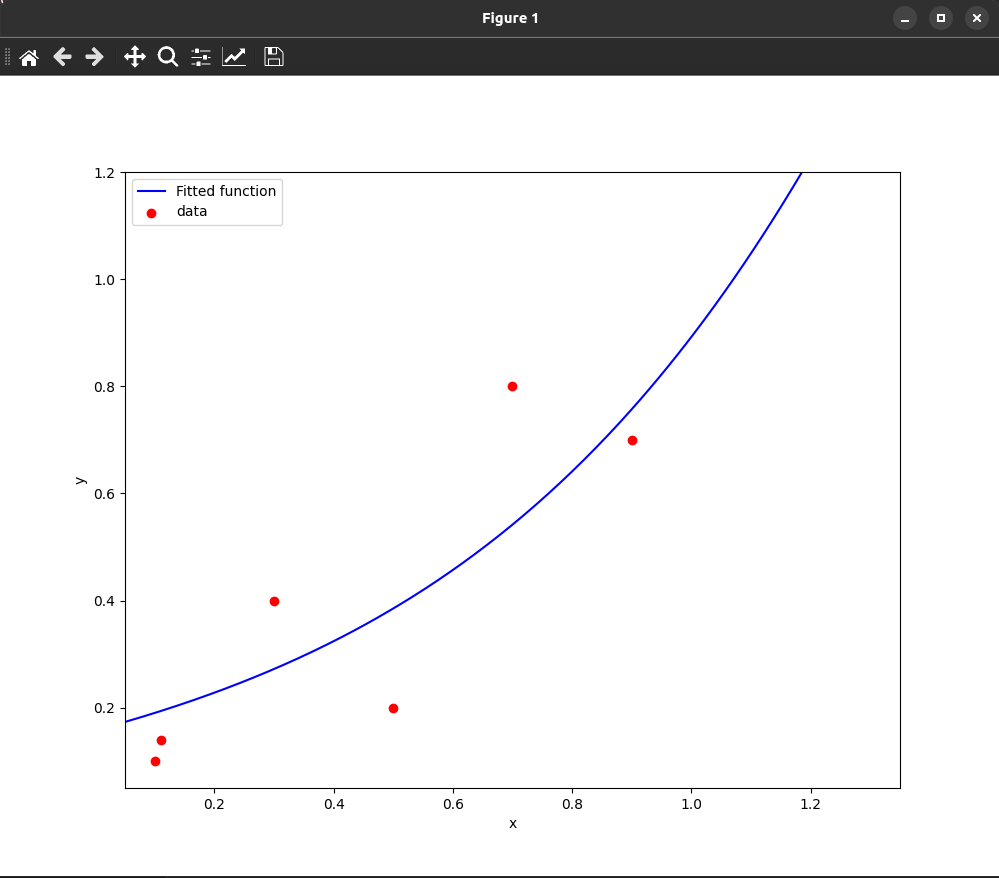
\includegraphics[width=9cm, height=7cm]{fit.png}
    \centering
    \caption{correção do overfitting anterior; mesmos settings,
    porém com regularization factor = $0.2$}
  \end{figure}

\section{Implementação}

\subsection{Design Matrix}

Essa matriz, em suma,contém os 
pontos do domínio do dataset após aplicar a polynomial
expansion. Portanto, suas dimensões são de:
$K$ por $\frac{(N+R-1)!}{R!(N-1)!}$, sendo $K$ o número de 
exemplos providenciados, e o número de colunas igual a
$C(N,R)$ (número de combinações com repetição para $N$
objetos e $R$ amostragens).

Visualmente, para uma transformação $\phi(x): \mathbb{R}^{D} 
\rightarrow \mathbb{R}^{K}$, a Design Matrix $\Phi(X)$ será
dada por:

$$
\Phi(X) = 
\begin{bmatrix}
    1 & \phi(x_{1}^{1}) & \phi(x_{2}^{1}) & ... & \phi(x_{N}^{1}) \\
    1 & \phi(x_{1}^{2}) & \phi(x_{2}^{2}) & ... & \phi(x_{N}^{2}) \\
    ... & ... & ... & ... & ... \\
    1 & \phi(x_{1}^{K}) & \phi(x_{2}^{K}) & ... & \phi(x_{N}^{K}) \\
\end{bmatrix}
$$

Onde os primeiros termos serem 1 satisfazem a necessidade de 
ter o termo independente $\theta_{0}$ de $f(x, \theta)$
(isso ficará mais claro em gradient descent), e 
a notação $x_{i}^{j}$ nesse caso indica que $x$ pertence à 
i-ésima dimensão do j-ésimo vetor de treinamento. Por exemplo,
para uma matriz com  3 vetores-exemplo de dimensão 2 em que 
deseja-se expandir polinomialmente até a terceira potência, 
teríamos:

$$
X = 
\begin{bmatrix}
    x_{1}^{1} & x_{2}^{1} \\
    x_{1}^{2} & x_{2}^{2} \\
    x_{1}^{3} & x_{2}^{3} \\
\end{bmatrix}
$$

$$
\Phi(X) = 
\begin{bmatrix}
    1 & x_{1}^{1} & x_{2}^{1} & (x_{1}^{1})^{2} & x_{1}^{1}x_{2}^{1} & (x_{2}^{1})^{2} \\
    1 & x_{1}^{2} & x_{2}^{2} & (x_{1}^{2})^{2} & x_{1}^{2}x_{2}^{2} & (x_{2}^{2})^{2}\\
    1 & x_{1}^{3} & x_{2}^{3} & (x_{1}^{3})^{2} & x_{1}^{3}x_{2}^{3} & (x_{2}^{3})^{2}\\
\end{bmatrix}
$$

A design matrix, no fim das contas, nada mais é além de
toda a informação necessária para treinar o modelo, já
que contém todos os vetores de treinamento do dataset, e
também apresenta-os expandidos ao grau que bem desejarmos.

\subsection{Gradient Descent}

A idéia básica do gradient descent é tentar minimizar a 
Loss Function descrita na equação \ref{eq:14} via o cálculo
do vetor gradiente, que aponta para a direção de máxima mudança
positiva na função (logo, basta invertê-lo para adquirir a 
direção de máxima mudança negativa). Tudo se resume a um
algoritmo muito simples:

\begin{enumerate}
    \item calcular $\nabla L(\theta,\lambda)$
    \item atualizar $\theta = \theta - \alpha
    \nabla L(\theta,\lambda)$
    \item repetir o processo para o mesmo $\Phi(X)$
\end{enumerate}

Algumas ressalvas importantes: 

\begin{itemize}
    \item o gradiente na verdade não 
    precisa ser necessariamente um vetor; ele pode ser um tensor
    de qualquer grau, sendo que ele só o é nesse caso graças 
    ao fato da regressão linear trabalhar com uma função
    $f:\mathbb{R}^{K} \rightarrow \mathbb{R}$ (generalizando:
    para $f:\mathbb{R}^{E} \rightarrow \mathbb{R}^{W}$,
    $\nabla f$ tem dimensões $W \times E$)
    \item $\alpha$ é a constante de aprendizado para a 
    atualização dos pesos. É necessário ajustar $\alpha$ com 
    cuidado: passos muito largos podem provocar overshooting,
    e os pequenos, demorarem demais para convergir ao ideal.
    \item apesar de muito famoso, o gradient descent não é
    único método iterativo para aproximação de extremos funcionais
    (quem diria); procure também pelo método de Newton.
\end{itemize}

É possível matematicamente provar que minimizar a função Loss já
descrita é equivalente a minimizar a clássica 'Mean Squared Error'.
Portanto, a fim de evitar ter de calcular $\sigma$, minimizaremos:

\begin{align}
    L(\theta, \lambda) &= \frac{1}{N}
    ||(Y - X\theta)||^{2} + \lambda
    ||\theta||_{2}^{2} \\
    &= \frac{1}{N}[\Sigma_{n=1}^{N}
    (y_{n} - x_{n}^{T}\theta)^{2}] + \lambda
    ||\theta||_{2}^{2} 
\end{align}

Dito isso, como fazemos o computador calcular esse gradiente?
Primeiro, é necessário calculá-lo manualmente:

\begin{align}
    \nabla L_{\theta} &= \frac{dL}{d\theta} \\
    &= \frac{2}{N}[\Sigma_{k=1}^{K}
    (y_{n} - \theta^{T}\phi(x_{n}))\phi(x_{n})]
    + 2\lambda \theta \\
    &= [\frac{\partial L}{\partial \theta_{1}}, 
    \frac{\partial L}{\partial \theta_{2}}, ...,
    \frac{\partial L}{\partial \theta_{K}}]
\end{align}

Daí em diante, baste seguir o algoritmo já descrito acima
para $\nabla L_{\theta}$, iterando até 
um ponto em que se estime já ser o suficiente.

\subsection{Complicações}

Como nem tudo são flores, durante o desenvolvimento desse projetinho,
passei por alguns apertos e indecisões (basta ver a evolução dos
meus commits). Abordarei aqui alguns problemas encontrados, que não
soube como solucionar:

\begin{itemize}
    \item \textbf{data range}: quanto maior a escala dos dados utilizados,
    menor tem que ser o $\alpha$ para evitar overflows numéricos, a
    um ponto em que a limitação do hardware para floating point 
    arithmetic impede o código de funcionar. Para solucionar isso,
    tentei usar data standardization e/ou normalization. Nenhum dos
    dois métodos funcionou, lamentavelmente, sendo isso um skill issue
    da minha parte.
    \item \textbf{questão do $\sigma$}: facilitar processamento,
    confesso, não foi a única razão pela qual optei por não 
    utilizar a Loss Function original. O livro que usei como base 
    (Mathematics for Machine Learning) apresentava a seguinte fórmula
    analítica para encontrar $\sigma$:
    \begin{equation}
        \sigma^{2} = \frac{1}{K}\Sigma_{k=1}^{K}
        (y_{n} - \theta^{T}\phi(x_{n}))^{2}
    \end{equation}
    porém, pelo que eu compreendi, a Loss Function seria:
    \begin{equation}
        L(\theta,\lambda,\sigma) = -\frac{1}{2\sigma^{2}}
        \Sigma_{k=1}^{K}
        (y_{n} - \theta^{T}\phi(x_{n}))^{2}
    \end{equation}
    Substituindo, teríamos:
    \begin{equation}
        L(\theta,\lambda,\sigma) = -\frac{K}{2}
    \end{equation}
    O que não faz o menor sentido. Se eu não entendo algo, eu não
    implemento.
\end{itemize}

\end{document}